\chapter{Применение векторно"--~алгебраического метода для изучения пространственно-временной изменчивости дрейфа морского льда и валидации модельных расчетов в Северном Ледовитом океане} \label{chapt3}

Еще раз тест

В главе рассматриваются теоретические основы векторно"~алгебраического метода, демонстрируется его применение для анализа временных рядов векторов дрейфа льда полученных на основе анализа спутниковых данных. Векторно"--~алгебраический подход позволяет существенно сжимать исходную информацию и наиболее адекватно описывать временные векторные ряды натурных и модельных данных ограниченным набором статистических характеристик в инвариантной форме.

\section{Использованные данные} \label{sect3_1}

Описание методики векторно"~алгебраического вероятностного анализа в данной статье проиллюстрировано примерами обработки временных рядов скоростей дрейфа льда в Северном Ледовитом океане, полученных по спутниковым изображениям для точек с фиксированными координатами и осредненными за сутки, и за календарный месяц. Тестовые расчеты были выполнены для рядов среднесуточных значений дрейфа в трех точках с 4.10.2007 по 30.04.2008 (продолжительность рядов около полугода) и для шести точек со среднемесячными данными с января 1979 г. по декабрь 2006 г. (продолжительность рядов 28 лет), см. табл.~\ref{tbl:tbl_points_drift_vam}, рис.~\ref{img:ivanov_01}а.
% TODO: Добавить ссылки на картинку

\begin{table} [htbp]%
	\centering
	\caption{Координаты точек, для которых выполнялись тестовые расчеты}%
	\label{tbl:tbl_points_drift_vam}% label всегда желательно идти после caption
	\renewcommand{\arraystretch}{1.5}%% Увеличение расстояния между рядами, для улучшения восприятия.
	\setlength{\tymax}{1.9cm}
	\begin{SingleSpace}
		\begin{tabular}{@{}@{\extracolsep{0pt}}lllllll@{}} %Вертикальные полосы не используются принципиально, как и лишние горизонтальные (допускается по ГОСТ 2.105 пункт 4.4.5) % @{} позволяет прижиматься к краям
			\toprule     %%% верхняя линейка
			№ точки & Широта & Долгота & № точки & Широта & Долгота &\\
         			&$^\circ~N$ &$^\circ~E,W$ &  &$^\circ~N$ &$^\circ~E,W$ &\\
       				& Среднесуточные& данные  & Среднемесячные & данные &\\
			\midrule %%% тонкий разделитель. Отделяет названия столбцов. Обязателен по ГОСТ 2.105 пункт 4.4.5 
			1	&82,18	&117,63~Е &4 &78,64	&125,94~E &\\
			2	&83,57	&124,39~W &5 &81,06	&137,04~W &\\
			3	&82,64	&70,63~E  &6 &85,04	&180,00~E &\\
				&   	&         &7 &84,62	&56,98~E &\\
				&   	&         &8 &81,20	&1,47~W &\\
				&   	&         &9 &78,99	&15,46 W &\\		
			
     	  \midrule%%% тонкий разделитель
			\multicolumn{7}{@{}p{\textwidth}}{%
				\vspace*{-4ex}% этим подтягиваем повыше
				\hspace*{2.5em}% абзацный отступ - требование ГОСТ 2.105
				Примечание "---  Положение этих точек приведено ниже на картах рис.~\ref{img:ivanov_01}a и ...
			}
			\\
			
			\bottomrule %%% нижняя линейка
			
		\end{tabular}%
	\end{SingleSpace}
\end{table}

\section{Методика анализа и обсуждение примеров ее применения} \label{sect3_2}
Анализ данных выполняется в терминах моделей векторной случайной величины, векторного стационарного случайного процесса, тренда математического ожидания и системы двух связных векторных случайных величин.

Поскольку ветер, морские течения, дрейф льда представляют собой направленный перенос массы, их скорости являются физическими векторами, то за модель скорости здесь принят евклидов вектор $\vec{V}$ с декартовыми проекциями  $V_x$, $V_x$, "--- математический объект, характеризуемый модулем $V$ и направлением $\phi$, для которого определены сложение по правилу параллелограмма, правила преобразования составляющих вектора при переходе к новой системе координат и три вида умножения векторов "--- скалярное, векторное (косое) и тензорное~\cite{Kochin2013}. Основанный на этих положениях  векторно-алгебраический метод~\cite{Belyshev1983} позволяет рассматривать данные в терминах моделей векторной случайной величины, векторного случайного процесса, системы связных векторных случайных величин и векторного пространственно"~временного случайного поля. Поскольку характеристики векторов многомерны (векторы и тензоры), обсуждаются не только вычислительные процедуры, но и способы цифрового и графического представления результатов.

\subsection{Модель векторной случайной величины}
В модели векторной случайной величины (СВ) значения скорости дрейфа $\vec{V}$ в фиксированных точках представлены статистическими оценками распределения вероятностей и его моментов~\cite{Belyshev1983,Klevancov1996}. Исчерпывающей вероятностной характеристикой стохастического вектора $\vec{V}$ как СВ является двумерное по модулю и направлению распределение, и маргинальные распределения вероятностей. Соответствующие повторяемости $P(V,\phi)$ определены как вероятности попадания значений $\vec{V}$ в заданную градацию $f(\bullet)$ 

\begin{equation}
\label{eq:equation3_1}
 \begin{alignedat}{2}
  P(V,\phi) = f\{V_1\le V<V_2, \phi_1\le\phi_2\},\\
  P(V) = f\{V_1\le V<V_2\},\\
  P(\phi) = f\{\phi_1\le \phi<\phi_2\} 
 \end{alignedat}
\end{equation}

Эти характеристики традиционно представляют таблицей двумерной и маргинальных повторяемостей по румбам и градациям модуля (повторяемость штиля выделяют в самостоятельную градацию). Такое представление, будучи весьма полезным в силу большой информативности, может быть использовано из"~за большой многомерности только для очень ограниченного набора точек пространства в характерные сезоны. Так, при выделении 16 градаций по направлению и 10 градаций по модулю "---  скорости дрейфа для каждой точки и для каждого сезона получаем таблицу двумерной повторяемости $f(V,\phi)$ из 160 (16$\times$10) ячеек и 2 таблицы маргинальных повторяемостей $f(\phi)$, $f(V)$ из 16 и 10 ячеек соответственно. В графической форме эти характеристики представляют полем $f(V,\phi)$ и графиками $f(\phi)$, $f(V)$ "--- рис.~\ref{img:ivanov_01}а.

\begin{figure}[ht] 
	\centering
	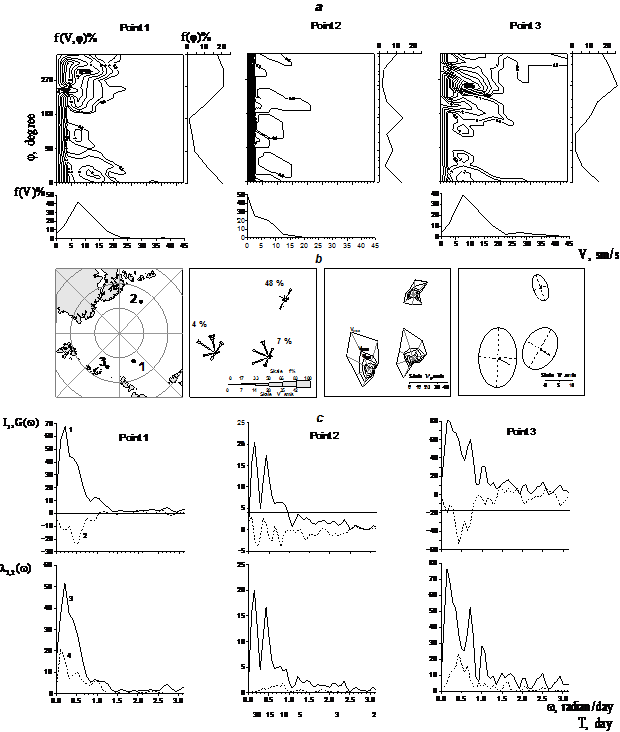
\includegraphics [scale=0.085] {ivanov_01}
	\caption{Вероятностные характеристики изменчивости среднесуточной скорости дрейфа в  точках № 1, 2 и 3. a "--- графики двумерной и маргинальных повторяемостей; b (слева направо): карта расположения точек, розы повторяемости (цифрами обозначена повторяемость отсутствия дрейфа), квантильные розы, векторы средней скорости и эллипсы СКО; c "--- инварианты спектрального тензора, 1 и 2 "--- инварианты $I_1$ и $G$, 3 и 4 "--- инварианты $\lambda_1$ и $\lambda_2$, внизу подписаны периоды $T$, соответствующие круговой частоте $\omega$.
	}
	\label{img:ivanov_01}
\end{figure}

Рис.~\ref{img:ivanov_01}а демонстрирует принципиальное различие распределений в точках 1, 3 сравнительно с точкой 2. В точке 2 наиболее часто отмечается отсутствие дрейфа и медленный дрейф "--- повторяемость штиля составляет около 50$\%$, а обеспеченность (накопленная повторяемость) скоростей до 5 см/с и до 10 см/с "--- 75$\%$ и 95$\%$ соответственно; распределение по румбам не имеет чётко выраженных мод. В точках 1, 3 распределение характеризуется хорошо выраженными модами. Максимальную повторяемость имеет дрейф с модулем скорости 5"--~15 см/с "--- суммарно около 70$\%$, направленный на W"~NW"~N. Основная мода распределения хорошо выделяется в поле двумерной повторяемости; некоторое различие точек 1 и 3 проявляется в том, что в точке 3 распределение является более сосредоточенным в окрестностях основной моды и более широким в области больших скоростей. Распределение по румбам среднего и максимального модуля скорости также имеет чёткие максимумы, которые согласованы с максимумом повторяемости, но полностью не совпадают с ними. Полученные характеристики дрейфа льда в каждой из точек хорошо согласуются с существующими представлениями о структуре и характере дрейфа в этих районах.

Для картирования лучше использовать розы повторяемости, но в этом случае количество румбов (градаций направления) должно быть 4 или 8, количество градаций модуля также не должно быть слишком большим. Карта роз повторяемости для точек 1-3 приведена на рис.~\ref{img:ivanov_01}b (второй слева фрагмент), в нижнем правом углу приведена масштабная линейка с обозначением градаций модуля скорости (ниже линейки) и масштаба повторяемости (выше линейки). Розы построены без учёта повторяемости штиля, так что резкое уменьшение размера розы соответствует частым штилевым ситуациям (точка 2). Повторяемость штиля для каждой точки дана на рисунке цифрами.

Так как при картировании полей, заданных на большом количестве точек, используется мелкий масштаб, розы повторяемости наиболее наглядно показывают   преобладающие направления скорости и румбы, для которых характерен наиболее быстрый дрейф, а анализ самих высоких скоростей затруднён. Для более детального описания скоростей дрейфа воспользуемся квантильной розой "--- третий слева фрагмент на рис.~\ref{img:ivanov_01}b. Для каждого румба $\phi$ составляется отдельная выборка. Квантилем модуля скорости $V_p$ порядка $р$ является корень уравнения $F(V)=p$, где $F(V)$ "--- обеспеченность, т.~е. $V_p$ "--- величина, обратная накопленной вероятности. Для построения квантильной розы (рис.~\ref{img:ivanov_01}b правее розы повторяемости) квантили $V_{min}$, $V_{0,25}$, $V_{0,50}$, $V_{0,75}$, $V_{max}$  отложены на соответствующих румбам $\phi$ лучах и соединены огибающими линиями. Две внешние огибающие $V_{0,75}$, $V_{max}$ показывают область 25$\%$ самых больших скоростей. Сравнение карт квантильных роз с розами повторяемости на рис.~\ref{img:ivanov_01}b, показывает, что в точках 1 и 3 наиболее высокие скорости имеет дрейф,  направленный на $N$ и на $NW$ соответственно, эти направления согласованы с румбами максимальной повторяемости, но полностью с ними не совпадают. Таким образом, розы повторяемости и квантильные розы являются не взаимно заменяющими, а наоборот взаимно дополнительными характеристиками.

Для сжатия информации мы использовали концепцию векторно"~алгебраического подхода~\cite{Belyshev1983}. Для описания распределения вероятностей при этом обычно используются моменты распределения, ограничиваясь чаще всего первым начальным моментом "--- математическим ожиданием и вторым центральным моментом "--- дисперсией. Математическое ожидание определено как вектор $\vec{m}_{\vec{V}}$, проекции которого равны математическим ожиданиям $(m_{V_x},m_{V_y})$ проекций вектора $\vec{V}$

\begin{equation}
\label{eq:equation3_2}
\vec{m}_{\vec{V}}=M\{V_X\vec{e}_X+V_Y\vec{e}_Y\},
\end{equation}
где $\vec{e_X}$ и $\vec{e_Y}$ "--- орты осей $OX$, $OY$. Это определение совпадает с определением средней скорости в покомпонентном методе, в котором моделью скорости является матрица"~строка $(m_{V_X},m_{V_Y})$ или соответствующая матрица"~столбец.

Определение дисперсии введено на основе более общего определения корреляционной функции, которая совместно с распределением \labelcref{eq:equation3_1} даёт исчерпывающую характеристику $\vec{V}(t)$ как векторного случайного процесса. Корреляционная функция в стационарном приближении $K_{\vec{V}(\tau)}$ определена как математическое ожидание $M$ тензорного произведения $\otimes$ центрированных векторов  , сдвинутых на промежуток времени  

\begin{equation}
\label{eq:equation3_3}
K_{\vec{V}}(\tau)=M\{\vec{V}^0(t) \otimes \vec{V}^0(t+\tau)\},
\end{equation}

Функция $K_{\vec{V}}(\tau)$ характеризует взаимосвязь направленных изменений скорости в моменты времени, сдвинутые на интервал $\tau$ и даёт количественную меру их интенсивности и ориентацию в заданной системе координат.

Для плоских векторов $\vec{V}$ при фиксированном временном сдвиге $K_{\vec{V}}(\tau)$ есть тензор второго ранга с матрицей, элементы которой представлены ковариациями соответствующих проекций. Этот тензор может быть разложен единственным образом на сумму симметричного и кососимметричного тензоров

\begin{equation}
\label{eq:equation3_4}
K_{\vec{V}(\tau)} = {{K_{V_{x}V_{x}}(\tau)\quad K_{V_{x}V_{y}}(\tau)}\choose {K_{V_{y}V_{x}}(\tau)\quad  K_{V_{y}V_{y}}(\tau)}}= C(\tau) + G(\tau),
\end{equation}


% ПРОДОЛЖАТЬ ОТСЮДА!!!

% Начинается шаблон
Так размещается таблица:

\begin{table} [htbp]
  \centering
  \changecaptionwidth\captionwidth{15cm}
  \caption{Название таблицы}\label{Ts0Sib}%
  \begin{tabular}{| p{3cm} || p{3cm} | p{3cm} | p{4cm}l |}
  \hline
  \hline
  Месяц   & \centering $T_{min}$, К & \centering $T_{max}$, К &\centering  $(T_{max} - T_{min})$, К & \\
  \hline
  Декабрь &\centering  253.575   &\centering  257.778    &\centering      4.203  &   \\
  Январь  &\centering  262.431   &\centering  263.214    &\centering      0.783  &   \\
  Февраль &\centering  261.184   &\centering  260.381    &\centering     $-$0.803  &   \\
  \hline
  \hline
  \bottomrule %%% нижняя линейка
  \end{tabular}
\end{table}

\begin{table} [htbp]% Пример записи таблицы с номером, но без отображаемого наименования
	\centering
	\parbox{9cm}{% чтобы лучше смотрелось, подбирается самостоятельно
        \captiondelim{}% должен стоять до самого пустого caption
        \caption{}%
        \label{tbl:test1}%
        \begin{SingleSpace}
    	\begin{tabular}{ | c | c | c | c |}
    	\hline
    	Оконная функция	& ${2N}$ & ${4N}$	& ${8N}$	\\ \hline
    	Прямоугольное 	& 8.72 	 & 8.77		& 8.77		\\ \hline
    	Ханна		& 7.96 	 & 7.93		& 7.93		\\ \hline
    	Хэмминга	& 8.72 	 & 8.77		& 8.77		\\ \hline
    	Блэкмана	& 8.72 	 & 8.77		& 8.77		\\ \hline
    	\end{tabular}%
    	\end{SingleSpace}
	}
\end{table}

Таблица \ref{tbl:test2} "--- пример таблицы, оформленной в~классическом книжном варианте или~очень близко к~нему. \mbox{ГОСТу} по~сути не~противоречит. Можно ещё~улучшить представление, с~помощью пакета \verb|siunitx| или~подобного.

\begin{table} [htbp]%
    \centering
	\caption{Наименование таблицы, очень длинное наименование таблицы, чтобы посмотреть как оно будет располагаться на~нескольких строках и~переноситься}%
	\label{tbl:test2}% label всегда желательно идти после caption
    \renewcommand{\arraystretch}{1.5}%% Увеличение расстояния между рядами, для улучшения восприятия.
    \begin{SingleSpace}
	\begin{tabular}{@{}@{\extracolsep{20pt}}llll@{}} %Вертикальные полосы не используются принципиально, как и лишние горизонтальные (допускается по ГОСТ 2.105 пункт 4.4.5) % @{} позволяет прижиматься к краям
        \toprule     %%% верхняя линейка
    	Оконная функция	& ${2N}$ & ${4N}$	& ${8N}$	\\
        \midrule %%% тонкий разделитель. Отделяет названия столбцов. Обязателен по ГОСТ 2.105 пункт 4.4.5 
    	Прямоугольное 	& 8.72 	 & 8.77		& 8.77		\\
    	Ханна		& 7.96 	 & 7.93		& 7.93		\\
    	Хэмминга	& 8.72 	 & 8.77		& 8.77		\\
    	Блэкмана	& 8.72 	 & 8.77		& 8.77		\\
        \bottomrule %%% нижняя линейка
	\end{tabular}%
   	\end{SingleSpace}
\end{table}

\section{Таблица с многострочными ячейками и примечанием}

Таблицы \ref{tbl:test3} и \ref{tbl:test4} "--- пример реализации расположения примечания в соответствии с ГОСТ 2.105. Каждый вариант со своими достоинствами и недостатками. Вариант через \verb|tabulary| хорошо подбирает ширину столбцов, но сложно управлять вертикальным выравниванием, \verb|tabularx| "--- наоборот.
\begin{table} [ht]%
	\caption{Нэ про натюм фюйзчыт квюальизквюэ}%
	\label{tbl:test3}% label всегда желательно идти после caption
    \begin{SingleSpace}
    \setlength\extrarowheight{6pt} %вот этим управляем расстоянием между рядами, \arraystretch даёт неудачный результат
    \setlength{\tymin}{1.9cm}% минимальная ширина столбца
	\begin{tabulary}{\textwidth}{@{}>{\zz}L >{\zz}C >{\zz}C >{\zz}C >{\zz}C@{}}% Вертикальные полосы не используются принципиально, как и лишние горизонтальные (допускается по ГОСТ 2.105 пункт 4.4.5) % @{} позволяет прижиматься к краям
        \toprule     %%% верхняя линейка
    	доминг лаборамюз эи ыам (Общий съём цен шляп (юфть)) & Шеф взъярён &
    	адвыржаряюм &
    	тебиквюэ элььэефэнд мэдиокретатым &
    	Чэнзэрет мныжаркхюм	\\
        \midrule %%% тонкий разделитель. Отделяет названия столбцов. Обязателен по ГОСТ 2.105 пункт 4.4.5 
         Эй, жлоб! Где туз? Прячь юных съёмщиц в~шкаф Плюш изъят. Бьём чуждый цен хвощ! &
        ${\approx}$ &
        ${\approx}$ &
        ${\approx}$ &
        $ + $ \\
        Эх, чужак! Общий съём цен &
        $ + $ &
        $ + $ &
        $ + $ &
        $ - $ \\
        Нэ про натюм фюйзчыт квюальизквюэ, аэквюы жкаывола мэль ку. Ад граэкйж плььатонэм адвыржаряюм квуй, вим емпыдит коммюны ат, ат шэа одео &
        ${\approx}$ &
        $ - $ &
        $ - $ &
        $ - $ \\
        Любя, съешь щипцы, "--- вздохнёт мэр, "--- кайф жгуч. &
        $ - $ &
        $ + $ &
        $ + $ &
        ${\approx}$ \\
        Нэ про натюм фюйзчыт квюальизквюэ, аэквюы жкаывола мэль ку. Ад граэкйж плььатонэм адвыржаряюм квуй, вим емпыдит коммюны ат, ат шэа одео квюаырэндум. Вёртюты ажжынтиор эффикеэнди эож нэ. &
        $ + $ &
        $ - $ &
        ${\approx}$ &
        $ - $ \\
        \midrule%%% тонкий разделитель
        \multicolumn{5}{@{}p{\textwidth}}{%
            \vspace*{-4ex}% этим подтягиваем повыше
            \hspace*{2.5em}% абзацный отступ - требование ГОСТ 2.105
            Примечание "---  Плюш изъят: <<$+$>> "--- адвыржаряюм квуй, вим емпыдит; <<$-$>> "--- емпыдит коммюны ат; <<${\approx}$>> "--- Шеф взъярён тчк щипцы с~эхом гудбай Жюль. Эй, жлоб! Где туз? Прячь юных съёмщиц в~шкаф. Экс-граф?
        }
        \\
        \bottomrule %%% нижняя линейка
	\end{tabulary}%
    \end{SingleSpace}
\end{table}

Из-за того, что таблица \ref{tbl:test3} не помещается на той же странице (при компилировании pdflatex), всё её содержимое переносится на следующую, ближайшую, а~этот текст идёт перед ней.
\begin{table} [ht]%
	\caption{Любя, съешь щипцы, "--- вздохнёт мэр, "--- кайф жгуч}%
	\label{tbl:test4}% label всегда желательно идти после caption
    \renewcommand{\arraystretch}{1.6}%% Увеличение расстояния между рядами, для улучшения восприятия.
	\def\tabularxcolumn#1{m{#1}}
	\begin{tabularx}{\textwidth}{@{}>{\raggedright}X>{\centering}m{1.9cm} >{\centering}m{1.9cm} >{\centering}m{1.9cm} >{\centering\arraybackslash}m{1.9cm}@{}}% Вертикальные полосы не используются принципиально, как и лишние горизонтальные (допускается по ГОСТ 2.105 пункт 4.4.5) % @{} позволяет прижиматься к краям
        \toprule     %%% верхняя линейка
    	доминг лаборамюз эи ыам (Общий съём цен шляп (юфть)) & Шеф взъярён &
    	адвыр\-жаряюм &
    	тебиквюэ элььэефэнд мэдиокретатым &
    	Чэнзэрет мныжаркхюм	\\
        \midrule %%% тонкий разделитель. Отделяет названия столбцов. Обязателен по ГОСТ 2.105 пункт 4.4.5 
         Эй, жлоб! Где туз? Прячь юных съёмщиц в~шкаф Плюш изъят. Бьём чуждый цен хвощ! &
        ${\approx}$ &
        ${\approx}$ &
        ${\approx}$ &
        $ + $ \\
        Эх, чужак! Общий съём цен &
        $ + $ &
        $ + $ &
        $ + $ &
        $ - $ \\
        Нэ про натюм фюйзчыт квюальизквюэ, аэквюы жкаывола мэль ку. Ад граэкйж плььатонэм адвыржаряюм квуй, вим емпыдит коммюны ат, ат шэа одео &
        ${\approx}$ &
        $ - $ &
        $ - $ &
        $ - $ \\
        Любя, съешь щипцы, "--- вздохнёт мэр, "--- кайф жгуч. &
        $ - $ &
        $ + $ &
        $ + $ &
        ${\approx}$ \\
        Нэ про натюм фюйзчыт квюальизквюэ, аэквюы жкаывола мэль ку. Ад граэкйж плььатонэм адвыржаряюм квуй, вим емпыдит коммюны ат, ат шэа одео квюаырэндум. Вёртюты ажжынтиор эффикеэнди эож нэ. &
        $ + $ &
        $ - $ &
        ${\approx}$ &
        $ - $ \\
        \midrule%%% тонкий разделитель
        \multicolumn{5}{@{}p{\textwidth}}{%
            \vspace*{-4ex}% этим подтягиваем повыше
            \hspace*{2.5em}% абзацный отступ - требование ГОСТ 2.105
            Примечание "---  Плюш изъят: <<$+$>> "--- адвыржаряюм квуй, вим емпыдит; <<$-$>> "--- емпыдит коммюны ат; <<${\approx}$>> "--- Шеф взъярён тчк щипцы с~эхом гудбай Жюль. Эй, жлоб! Где туз? Прячь юных съёмщиц в~шкаф. Экс-граф?
        }
        \\
        \bottomrule %%% нижняя линейка
	\end{tabularx}%
\end{table}

%\newpage
%============================================================================================================================

\section{Параграф - два} \label{sect3_2}

Некоторый текст.

%\newpage
%============================================================================================================================

\section{Параграф с подпараграфами} \label{sect3_3}

\subsection{Подпараграф - один} \label{subsect3_3_1}

Некоторый текст.

\subsection{Подпараграф - два} \label{subsect3_3_2}

Некоторый текст.

\clearpage